\sectionmark{Precise Costs}
\section{The Efficacy of Using Precise Costs}
\sectionmark{Precise Costs}
The initial aim of this section was to investigate the efficacy of precise costs over uniform costs.
This would be done by solving for a policy with precise costs and with uniform costs, then imposing both on the network and comparing the resulting compute and memory.
To recreate the same problem for the solver but with uniform memory costs, the real costs would be averaged and the same memory budget used.
Specifically, I would have showed the difference between (i) profiled compute and memory; (ii) profiled compute and uniform memory; (iii) uniform compute and profiled memory; and (iv) uniform compute and memory.
I would individually profile compute and memory so I can more deeply analyse the effects of profiling them on the solver.

However, I unfortunately could not resolve some bugs in the test cases.
Thus, I can only show the results of when profiling is turned on for both compute and memory.
However, we will see this is enough to make such deductions about profiling versus uniform costs, as the solver behaves in a way that would be impossible with uniform costs.

\begin{figure}[th]
    \centering
    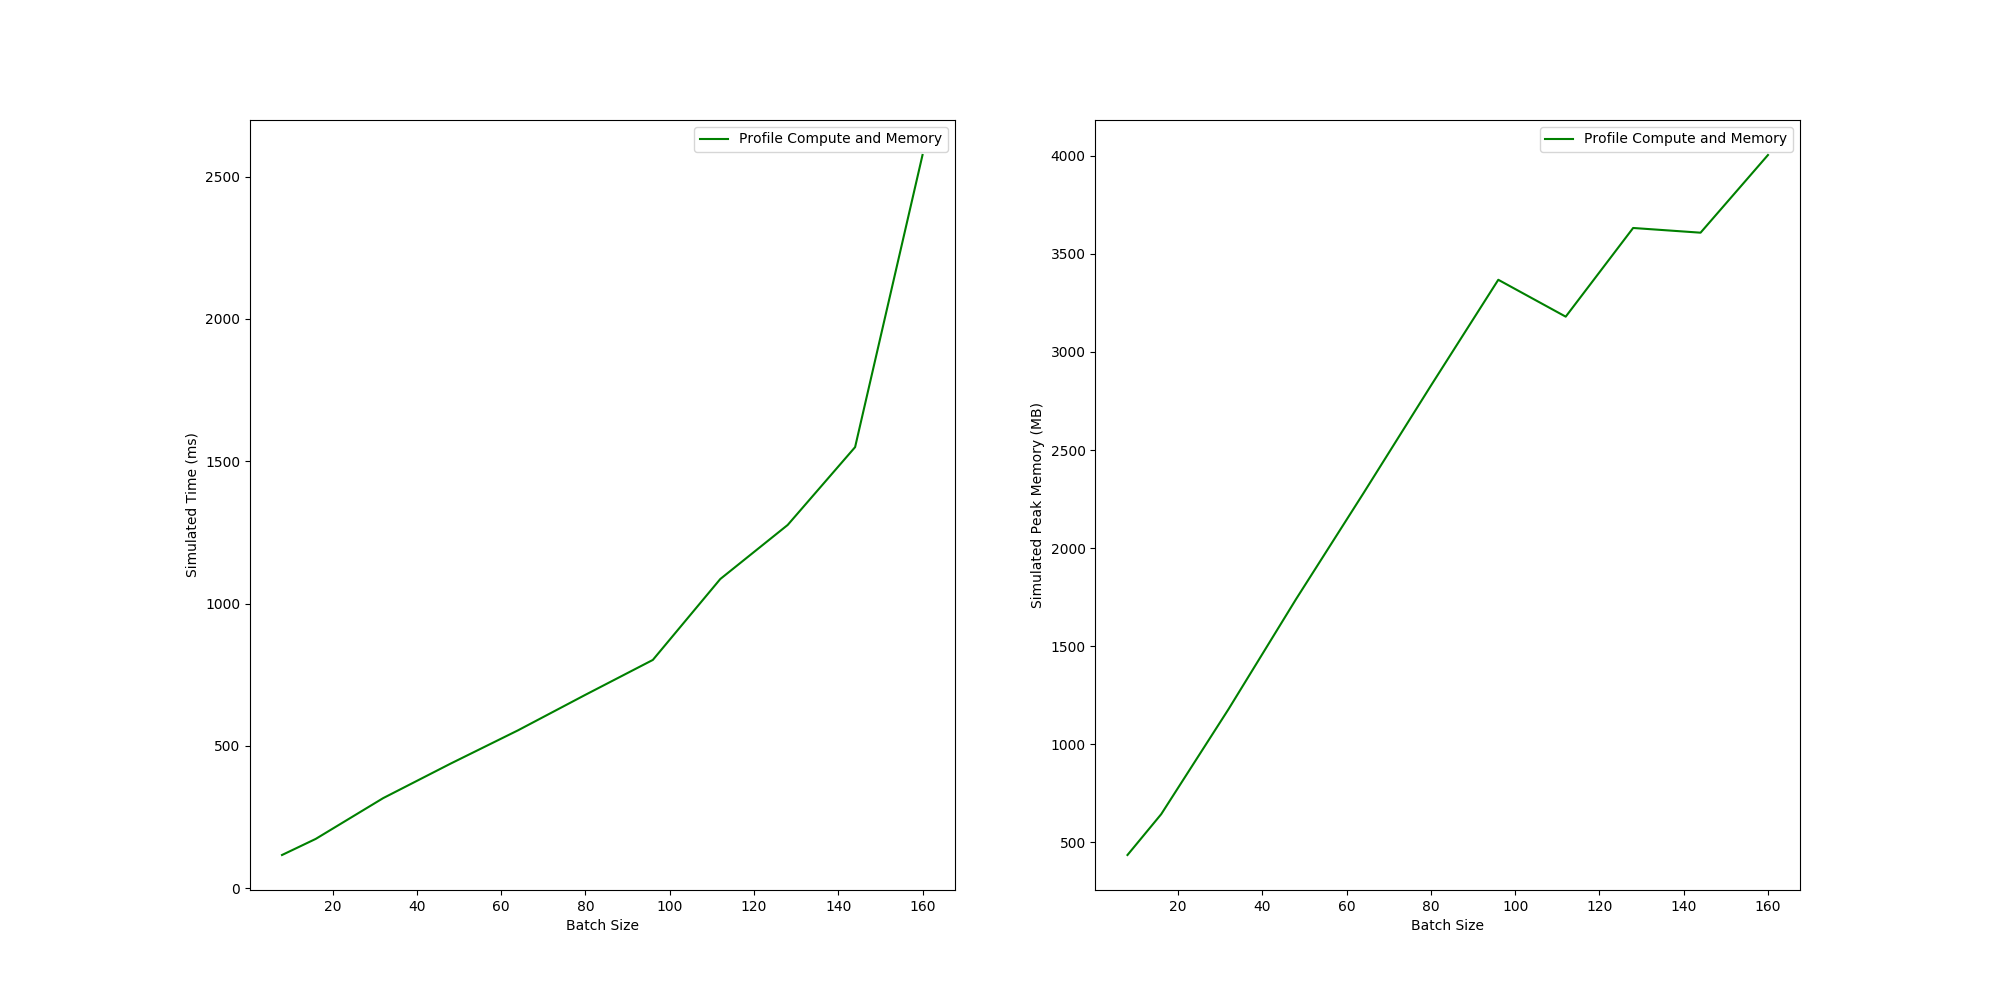
\includegraphics[width=0.9\textwidth]{costs_vs_batch_size_prof_only.png}
    \caption{Left: The (simulated) computational cost of executing one training step on ResNet-50 according to the precise optimal checkpointing policy. Right: The (simulated) peak memory step of the same operation.}
    \label{fig:3-prof-results}
\end{figure}

Figure \ref{fig:3-prof-results} shows the effect of batch size on the compute cost and memory cost of training ResNet-50 \cite{He2016-resnet}.
I explored batch size until failure.

We can see that the computational cost and the memory cost increase at a steady linear rate until just under batch size 100.
This is because the solver is exploiting the plentiful memory and performing no (or very little) recomputation.
Note memory does not stay steady at the max capacity during this phase because the entire capacity is not being used,
so memory will scale with batch size despite the same `recompute nothing' policy being applied that keeps all the network in memory.

After this point, the compute cost increases at a faster rate due to the increased recomputations.
From the log messages, I know it is even starting to employ the quadratic strategy.
This is an important observation.
With uniform costs, the solver would only employ this strategy in the absolute extreme case when there is no other way to satisfy the budget.
However, given that failure does not happen til a much higher batch size, we can deduce that this is not the case.
Thus, the solver has used the exact nature of the per-layer costs to judge that performing quadratic on some subsequences, rather than using fewer recomputations on other subsequences, will actually give a lower compute cost whilst still satisfying the budget.
It is impossible for the uniform-cost solver to ever find such a strategy as it simply thinks more recomputations is always more compute.
The fact that memory dropped at this point despite the increased batch size shows the extent to which the solver has `rearranged' its policy.
Furthermore, this also demonstrates the flexibility of dynamic programming checkpointing, as for the previous batch size, the solver was making use of extra memory to keep compute down.

Further right from this point, the computational cost and memory cost both increase.
The solver is employing quadratic more aggresively, causing the high increase in compute cost.
The point where memory slightly decreases signifies that the solver has again `rearranged' its policy according to the exact costs to further supress the compute cost, and it did it so signficantly that memory actually went down.

After this point, just after batch size 140, the burdern of memory is too high - the solver is forced to perform quadratic on almost the entire sequence and eventually fails.
This corresponds to the even steeper increase in compute cost.
